%%%%%%%%%%%%Outline%%%%%%%%%%%%%%%%%%

% Section 4 overview

% message<Section 4 explains the design of BpfReJIT as a post-load optimization loop: how it recompiles a live program, how rewritten programs can use new native instructions, how rewrites are chosen, and why the kernel remains the final safety boundary.>

% 4.1 Recompiling a Live Program

% message<BpfReJIT treats optimization as recompilation of the same live program, not replacement by a different program.>
% message<This design therefore needs both a stable rewrite baseline and an in-place replacement path.>
% message<Together, these two properties make live optimization transparent to existing attachments and links.>

% 4.2 Exposing New Native Instructions

% message<Recompiling a live program is useful only if the rewritten program can produce better native code than plain BPF rewriting allows.>
% message<BpfReJIT therefore lets the kernel expose additional native instructions that rewritten programs may use.>
% message<This design expands what recompilation can produce without moving optimization policy into the kernel.>

% 4.3 Choosing Rewrites in Userspace

% message<Once the kernel exposes multiple legal rewrite choices, selecting among them becomes a policy problem rather than a safety problem.>
% message<BpfReJIT assigns that policy problem to a userspace daemon that closes the optimization loop for live programs.>
% message<This split keeps rewrite selection adaptable to workload and deployment context while leaving the kernel interface stable.>

% 4.4 Keeping the Kernel as the Safety Boundary

% message<BpfReJIT works because kernel safety and rewrite correctness are separate responsibilities.>
% message<The kernel remains the final safety gate for every rewritten program, while the daemon is responsible for semantic preservation.>
% message<This boundary makes repeated live optimization fail-safe because rejected rewrites change nothing and accepted rewrites preserve program identity.>

%%%%%%%%%%%%Outline%%%%%%%%%%%%%%%%%%

\section{BPF Recompilation Framework}
\label{sec:rejit}

Figure~\ref{fig:workflow} shows the workflow of \tool. \tool adds a post-load optimization loop without changing the normal eBPF execution path. Once a program is loaded and attached, the kernel saves its original bytecode and keeps running the current JIT code on the normal fast path. A privileged userspace daemon discovers live programs, reads their original bytecode and runtime information, rewrites a whole program, and sends the rewritten version back to the kernel. The kernel then re-verifies and re-JITs that rewritten program and, if both steps succeed, atomically replaces the JIT code for the same logical program. This split lets the daemon decide which rewrites are profitable, while the kernel decides which rewrites are legal and safe. The rest of this section explains the three parts that make this loop work: reading and replacing live programs, exposing new instruction targets, and choosing rewrites in userspace.

\begin{figure}[hbtp]
    \centering
    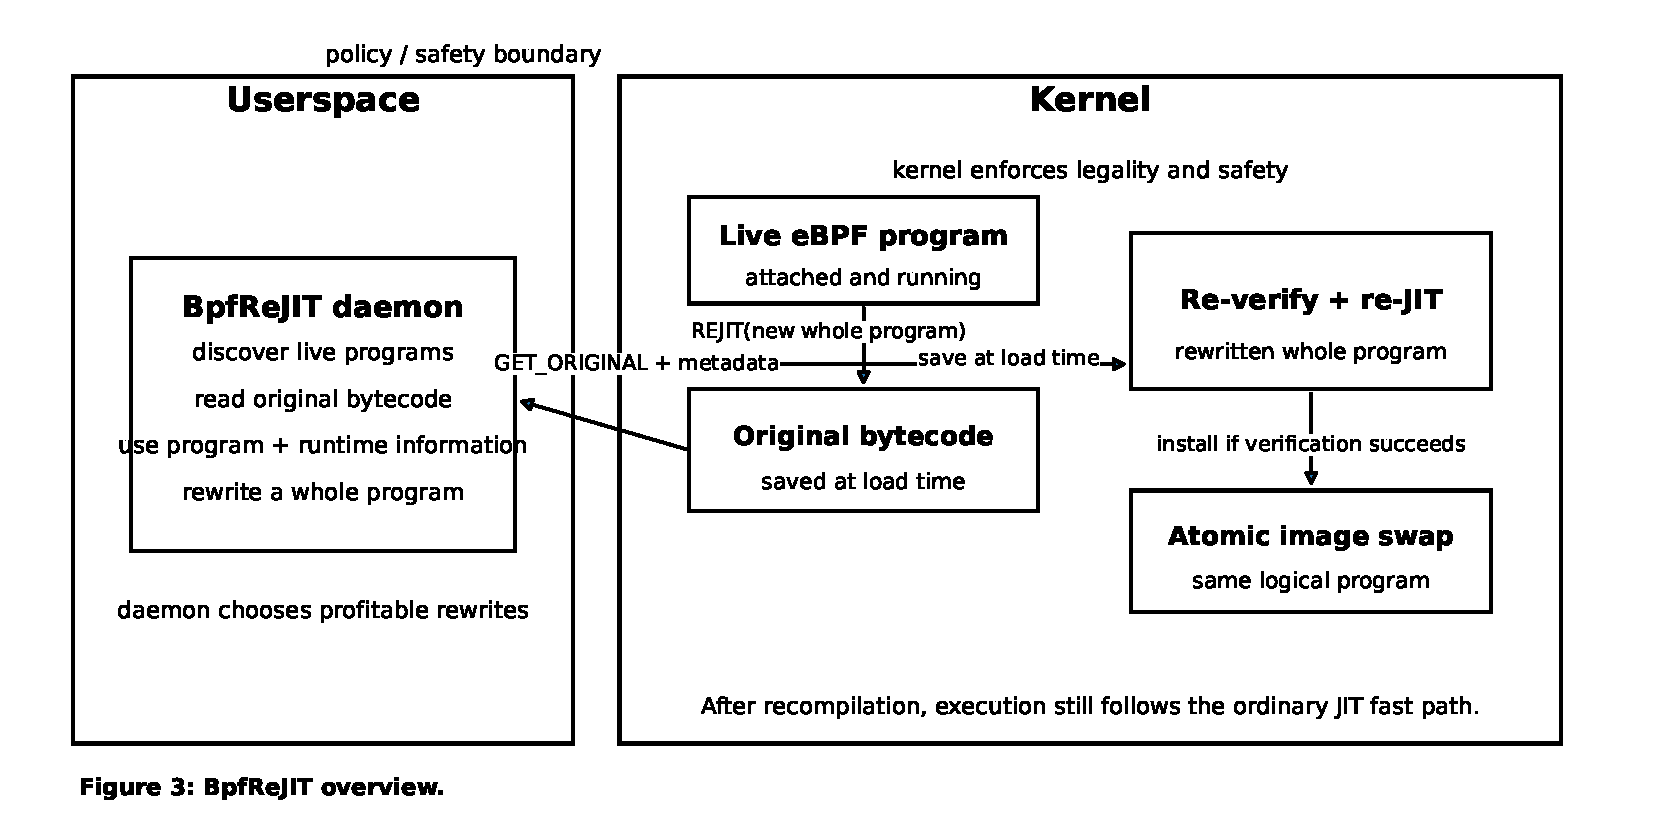
\includegraphics[width=1\linewidth]{figures/architecture-overview.pdf}
    \caption{Overview of \tool. The daemon reads a live program, rewrites a whole program in userspace, and sends it back to the kernel; the kernel re-verifies, re-JITs, and replaces the JIT code in place. After recompilation, execution still follows the ordinary JIT fast path.}
    \label{fig:workflow}
\end{figure}

\subsection{Overall Workflow}
\label{sec:rejit-overall}

\noindent\textbf{Starting from the original program.} Recompilation begins from the original bytecode of a live program rather than from translated instructions or an existing JIT image. This choice gives the daemon a stable whole-program baseline on which to analyze and rewrite the program. The daemon first identifies a target live program and retrieves its original eBPF bytecode together with the metadata needed to rebuild a complete candidate. Reconstructing each optimization attempt from the same logical baseline avoids the fragility of incrementally patching already transformed code and ensures that every recompilation starts from a representation whose semantics match the originally loaded program.

\noindent\textbf{Whole-program rewriting in userspace.} The daemon rewrites the recovered program through a pass pipeline that operates on extended eBPF. We group these passes into three broad classes. The first class performs normalization and BPF-to-BPF simplification, such as canonicalizing control flow or exposing patterns that later passes can reason about more easily. The second class introduces kinsn by recognizing bytecode idioms whose semantics can be represented more directly in the extended bytecode defined in Section~\ref{sec:kinsn}. The third class performs runtime specialization by materializing facts learned after deployment and propagating the resulting simplifications through the rest of the program. A practical specialization pipeline may combine map-value materialization, constant propagation, and dead-code elimination into one whole-program rewrite. Regardless of the specific passes selected, the daemon always produces a complete candidate program $P'$ rather than a patch against the currently installed image.

\subsection{Deployment Model}
\label{sec:rejit-deployment}

\noindent\textbf{Apply-all mode.} In apply-all mode, the daemon enumerates the currently loaded eBPF programs, reconstructs each candidate from its original bytecode, applies the selected pass pipeline, and exits after one optimization round. This mode is useful for controlled experiments and benchmarking because it produces a deterministic before-and-after comparison over a fixed set of live programs.

\noindent\textbf{Watch mode.} In watch mode, the daemon remains resident and applies the same workflow continuously as new programs are loaded or as runtime conditions justify re-specialization. This mode is the natural deployment model for production systems. It preserves transparency for existing applications while allowing optimization policy to evolve in userspace, where pass selection, specialization thresholds, and rollback policy can be updated without changing the kernel interface. In both modes, the underlying mechanism is the same: reconstruct from original bytecode, rewrite the whole program in extended eBPF, re-verify through proof lowering, and install the new native image only if the kernel accepts it.